% Part 2 chapter (replaces the electron section of p2_15_particle_masses.tex). Carries "Electron Rest Mass from Holographic Horizon
% Thermodynamics" (Feb 2026; docs/papers/Electron_Rest_Mass_from__IAM.pdf, PDF text 475 lines, and its source electron_mass_referee_safe.tex,
% 486 lines; both read in full 2026-10-02). Corrections: PAPER_ERRATA EM1-EM4 and EM5-EM8 (MANIFEST_particle.md). Numbers:
% docs/verification/scripts/verify_particle_book.py (E1-E12) and verify_electron_mass.py. Figure: docs/book/figscripts/fig_p2_particle.py.
\chapter{The electron rest mass as a fixed point}\label{ch:electronmass}

\section*{The place}
The electron mass is an input of the Standard Model, set by a Yukawa coupling $y_e=\sqrt2m_e/v=2.9\times10^{-6}$ (Chapter~\ref{ch:higgsrecord}).
This chapter asks whether IAM's Law (Chapter~\ref{ch:iams_law}) can read it instead as a fixed point: the mass at which the electron's rest energy
equals the cost of keeping its own record, priced at the temperature of the cosmic horizon. The equation is set out factor by factor. Its
solution falls short of the electron mass by a factor $1.74$ until one further factor, found by numerical search, is included. With that factor
the result agrees with the measured mass within the $0.3\,\%$ that the uncertainty of $H_0$ allows. The chapter states which factors are derived,
which are assumed and which was identified numerically.

\section{One temperature formula, two horizons}\label{sec:em:horizons}
A horizon of surface gravity $\kappa$ has temperature
\begin{equation}
T=\frac{\hbar\kappa}{2\pi\kB}\label{eq:em:T}
\end{equation}
(Eq.~\eqref{eq:ko:TU}). For a Schwarzschild black hole $\kappa=c^3/4GM$ and $T_H=\hbar c^3/8\pi GM\kB$~\cite{Hawking1975}; for the de Sitter horizon
$\kappa=H$ and $T_{GH}=\hbar H/2\pi\kB$~\cite{GibbonsHawking1977}. In both the $2\pi$ is the Euclidean period of the near-horizon geometry. \derived{}
At $H_0=67.4$\,km\,s$^{-1}$\,Mpc$^{-1}$ the cosmic horizon is at $T_{GH}=2.66\times10^{-30}$\,K. \calc

\section{The ingredients}\label{sec:em:ingredients}
\paragraph{The encoding surface.} The electron of mass $m$ is assigned its reduced Compton sphere, radius $\bar\lambda_C=\hbar/mc$, as the surface
on which its record is kept, with the area count of a horizon of that size:
\begin{equation}
S=\frac{4\pi\bar\lambda_C^2}{4\lP^2}=\pi\Big(\frac{\mP}{m}\Big)^2=1.79\times10^{45}\quad(m=m_e).\label{eq:em:S}
\end{equation}
\conjecture{} This is the area law applied to the Compton sphere. It is not saturation of Bekenstein's bound. That bound, $S\le2\pi ER/\hbar c$ for
energy $E$ in radius $R$~\cite{Bekenstein1981}, gives $S\le2\pi$ for $E=mc^2$ and $R=\bar\lambda_C$, smaller than Eq.~\eqref{eq:em:S} by a factor
$2.9\times10^{44}$. \calc{} A sphere of radius $\bar\lambda_C$ reaches the area count only if it holds the mass of a black hole of that size.

\paragraph{The price of a bit.} Each bit is priced by IAM's Law at the temperature of the cosmic horizon,
\begin{equation}
E_{\rm bit}=\kB T_{GH}\ln2=\frac{\hbar H_0\ln2}{2\pi}=2.54\times10^{-53}\ {\rm J}.\label{eq:em:Ebit}
\end{equation}
\derived{} (given IAM's Law and the choice of the cosmic horizon as the pricing surface). $H_0$ enters as today's value. The Compton sphere keeps
the record; the cosmic horizon sets its price.

\paragraph{The cell count.} The number of encoding cells is taken to scale as
\begin{equation}
N(m)=\Big(\frac{\mP}{m}\Big)^{3/2}=\Big(\frac S\pi\Big)^{3/4}=3.69\times10^{33}\quad(m=m_e).\label{eq:em:N}
\end{equation}
\conjecture{} The exponent $3/2$ is argued from dimensional homogeneity and the virial partition of a $1/r$ potential. Fixing it is open.
$\mP/m$ is dimensionless, so every power of it is dimensionally homogeneous. The virial half (Chapter~\ref{ch:virial}) fixes the ratio of kinetic
to potential energy in a $1/r$ potential; it does not fix how a cell count scales with mass. \derived{} The coefficient of $N$ is set to 1.

\paragraph{The electromagnetic factor.} A charged particle is taken to write gravitationally at a rate reduced by a factor $f(\alpha)$, given two
ways. Spatially: the Coulomb self-energy $e^2/4\pi\varepsilon_0r$ equals $mc^2$ at the classical radius $r_e=\alpha\bar\lambda_C$ and equals
$\alpha mc^2$ at $\bar\lambda_C$~\cite{PDG2024}. \observed{} The fraction of cells taken by the electromagnetic encoding is set to
$(r_e/\bar\lambda_C)^{3/2}=\alpha^{3/2}$, and the energy diverted from the gravitational record to $\alpha$, so
\begin{equation}
f(\alpha)\big|_{\rm spatial}=\alpha^{3/2}\cdot\alpha=\alpha^{5/2}=4.55\times10^{-6}.\label{eq:em:fs}
\end{equation}
Temporally: with the Compton time $\tau_C=\hbar/mc^2$ and $\tau_{\rm EM}=\hbar/\alpha mc^2=\tau_C/\alpha$, the gravitational rate is diluted by
$\alpha$, and the electromagnetic orbit occupies $(\tau_{\rm EM}/\tau_C)^{3/2}=\alpha^{-3/2}$ modes, so
\begin{equation}
f(\alpha)\big|_{\rm temporal}=\alpha\cdot\alpha^{3/2}=\alpha^{5/2}.\label{eq:em:ft}
\end{equation}
\conjecture{} The two arguments agree because both multiply one factor of $\alpha$ by the same $3/2$ power. The $3/2$ is taken from
Eq.~\eqref{eq:em:N}; it is not the exponent of a volume ratio, which for lengths would be 3. The agreement is a consistency of the two readings,
not an independent derivation.

\section{The fixed point and its solution}\label{sec:em:fixed}
The electron is taken to be a stable, self-consistent record: its rest energy equals the cost of maintaining it,
\begin{equation}
mc^2=E_{\rm bit}\,\frac{N(m)}{f(\alpha)}.\label{eq:em:fp}
\end{equation}
\conjecture{} The mass appears on both sides. The left side grows as $m$, the right side falls as $m^{-3/2}$, so there is exactly one positive
solution (Figure~\ref{fig:em:fp}a). \derived{} Substituting Eqs.~\eqref{eq:em:Ebit}, \eqref{eq:em:N} and \eqref{eq:em:fs},
\begin{equation}
mc^2=\frac{\hbar H_0\ln2}{2\pi}\cdot\frac{(\mP/m)^{3/2}}{\alpha^{5/2}}\quad\Longrightarrow\quad
m^{5/2}=\frac{\hbar H_0\ln2\;\mP^{3/2}}{2\pi\,\alpha^{5/2}c^2},\label{eq:em:m52}
\end{equation}
and
\begin{equation}
m_*=(2\pi)^{-2/5}\,\mathcal B,\qquad\mathcal B\equiv\left[\frac{\hbar H_0\ln2\;\mP^{3/2}}{\alpha^{5/2}c^2}\right]^{2/5}.\label{eq:em:mstar}
\end{equation}
\derived{} (given the ingredients). At $H_0=67.4$, $\mathcal B=1.2018\,m_e$ and $(2\pi)^{-2/5}=0.4794$, so the fixed point as derived is
\begin{equation}
m_*=0.5762\,m_e.\label{eq:em:short}
\end{equation}
\calc{} At the true electron mass the right side of Eq.~\eqref{eq:em:fp} is $0.252\,m_ec^2$, a factor $3.97$ short (E9). \calc

\paragraph{The identified factor.} The measured mass is reached with the prefactor $(2\pi)^{-1/10}$ in place of $(2\pi)^{-2/5}$:
\begin{equation}
m_e=(2\pi)^{-1/10}\left[\frac{\hbar H_0\ln2\;\mP^{3/2}}{\alpha^{5/2}c^2}\right]^{2/5}=1.0000066\,m_e\quad(H_0=67.4).\label{eq:em:result}
\end{equation}
The needed prefactor is $0.832107$; $(2\pi)^{-1/10}=0.832112$. \calc{} Of $(2\pi)^{-1/10}$, the part $(2\pi)^{-2/5}$ comes from $T_{GH}$ through
the $2/5$ root. The rest, $(2\pi)^{3/10}=1.7356$, was found by a numerical search among simple combinations of constants. \fitted{} It is
equivalent to a coefficient $(2\pi)^{3/4}=3.969$ in the cell count, $N=(2\pi)^{3/4}(\mP/m)^{3/2}$; that restates the factor; deriving it is open. \calc{} A geometric origin has been proposed: the null path from the Compton sphere to the de Sitter horizon in the static patch, continued to
Euclidean time, would subtend a quarter of the thermal circle. An integral that turns this into $(2\pi)^{3/10}$ is the next step; searches by Cauchy projection, Stefan--Boltzmann exchange between the two horizons, $S^4$ volume integration and near-horizon mode counting have not yet produced it. \openprob

\begin{table}[htbp]\centering\small
\caption{The factors of the electron fixed point at $H_0=67.4$\,km\,s$^{-1}$\,Mpc$^{-1}$. CODATA constants (via \texttt{scipy.constants});
\texttt{verify\_particle\_book.py} (E1--E9).}\label{tab:em:factors}
\begin{tabular}{llll}\toprule
factor & expression & value & label\\\midrule
bit price & $\hbar H_0\ln2/2\pi$ & $2.54\times10^{-53}$\,J & \derived\\
area count of the Compton sphere & $\pi(\mP/m_e)^2$ & $1.79\times10^{45}$ & \conjecture\\
Bekenstein bound for $m_ec^2$ in $\bar\lambda_C$ & $2\pi$ & $6.28$ & \derived\\
cell count & $(\mP/m_e)^{3/2}$ & $3.69\times10^{33}$ & \conjecture\\
electromagnetic factor & $\alpha^{5/2}$ & $4.55\times10^{-6}$ & \conjecture\\
bracket & $\mathcal B/m_e$ & $1.2018$ & \calc\\
fixed point as derived & $(2\pi)^{-2/5}\mathcal B/m_e$ & $0.5762$ & \calc\\
identified factor & $(2\pi)^{3/10}$ & $1.7356$ & \fitted\\
with the identified factor & $(2\pi)^{-1/10}\mathcal B/m_e$ & $1.0000066$ & \calc\\\bottomrule
\end{tabular}
\end{table}

\begin{figure}[htbp]\centering
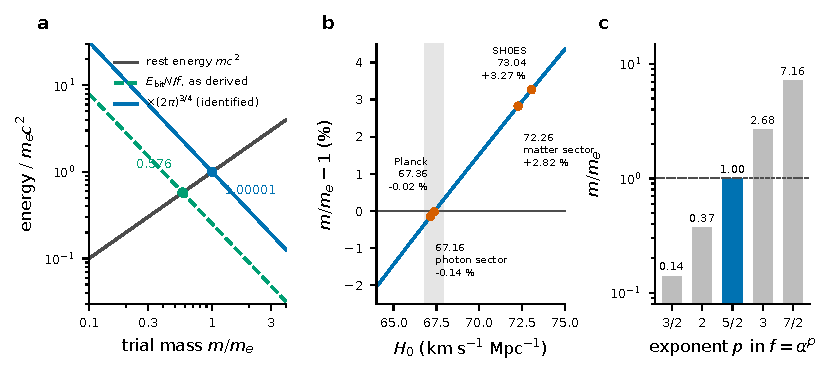
\includegraphics[width=\textwidth]{figures/part2/fig_electron_fp.pdf}
\caption[The electron fixed point]{(a) The two sides of Eq.~\eqref{eq:em:fp} against a trial mass, in units of $m_ec^2$: the rest energy (grey),
the cost $E_{\rm bit}N/f$ as derived (green, dashed; crossing at $0.576\,m_e$) and with the identified factor $(2\pi)^{3/4}$ in $N$ (blue; crossing at
$1.00001\,m_e$), $H_0=67.4$. (b) The fixed point with the identified factor against $H_0$: $-0.14\,\%$ at the photon-sector $67.16$, $-0.02\,\%$ at the
Planck $67.36$ (band: $\pm0.54$), $+2.82\,\%$ at the matter-sector $72.26$ and $+3.27\,\%$ at the SH0ES $73.04$~\cite{Planck2018VI,Riess2022}. (c) The
fixed point with the identified factor for other exponents $p$ of $f=\alpha^p$: only $p=5/2$, the exponent at which the factor was found, gives
$m_e$; $p=7/2$ gives $7.16\,m_e$. CODATA constants. Panel (a) and (c) \calc; the identified factor \fitted.}\label{fig:em:fp}
\end{figure}

\section{The precision set by $H_0$}\label{sec:em:H0}
The fixed point scales as $m_e\propto H_0^{2/5}$. Its precision is that of $H_0$: the Planck uncertainty $\sigma(H_0)=0.54$~\cite{Planck2018VI}
alone gives $\pm0.32\,\%$ in $m_e$. \calc{} The identified factor was found at $H_0=67.4$, and Eq.~\eqref{eq:em:result} is exact at $H_0=67.399$.
The 6.6\,ppm agreement at $67.4$ is therefore fixed by that choice and carries no information beyond it. \calc{} Stated at the precision the inputs
allow: the fixed point lands on the electron mass within the $0.3\,\%$ set by $H_0$, with one factor identified numerically.

\begin{center}\small\begin{tabular}{lll}\toprule
$H_0$ (km\,s$^{-1}$\,Mpc$^{-1}$) & source & $m/m_e-1$\\\midrule
67.16 & photon sector (Chapter~\ref{ch:dual}) & $-1419$\,ppm\\
67.36 & Planck 2018 best fit~\cite{Planck2018VI} & $-231$\,ppm\\
67.40 & value at which the factor was identified & $+7$\,ppm\\
72.26 & matter sector (Chapter~\ref{ch:dual}) & $+2.82\,\%$\\
73.04 & SH0ES~\cite{Riess2022} & $+3.27\,\%$\\\bottomrule
\end{tabular}\end{center}
\calc{} The two sector values of the framework give different answers. With the photon-sector $67.16$ the fixed point is $0.14\,\%$ low, inside
the $0.32\,\%$ spread. With the matter-sector $72.26$ it is $2.8\,\%$ high, nearly nine times that spread. Which expansion rate prices the bit is
not stated by the ingredients; the background horizon, which the framework leaves unmodified, is the natural candidate, and with it the
agreement holds. \openprob

\section{The exponent $5/2$}\label{sec:em:exponent}
Part~\ref{part:2}'s integral check tests whether the exponent $5/2$ of $\alpha$ is also the exponent that sets the rate of cosmic information production, $D(a)^{5/2}$. With the full $\Lambda$CDM growth factor, a source term $D^{5/2}\Omega_mf/T_H$ gives
$E(a)\propto\exp(0.76-0.87/a)$, not $\exp(1-1/a)$; the activation function is recovered to within $5\,\%$ by $D^{7/2}$
(Chapter~\ref{ch:theory}, Section~\ref{sec:numerics}). \calc{} The cosmology takes $7/2$; the electron's $5/2$ rests only on the arguments of
Eqs.~\eqref{eq:em:fs}--\eqref{eq:em:ft}. Whether the two exponents are related is open (Chapter~\ref{ch:nonlocal}). \openprob

Inside the electron formula the exponent and the identified factor are not separate. With $(2\pi)^{-1/10}$ held fixed, $p=3/2$, 2, 5/2, 3 and
7/2 give $0.14$, $0.37$, $1.00$, $2.68$ and $7.16\,m_e$ (Figure~\ref{fig:em:fp}c): $m\propto\alpha^{-2p/5}$, so each half-step in $p$ is a factor
$\alpha^{-1/5}=2.68$. \calc{} The factor was found with $p=5/2$ in place, so this table shows how tightly the two are tied; whether the data select $5/2$ on their own is the open question.

\section{Two temperatures}\label{sec:em:temps}
The fixed point can be read as a balance between two thermal surfaces: the Compton sphere at $T_C=m_ec^2/2\pi\kB=9.44\times10^8$\,K and the cosmic
horizon at $T_{GH}=2.66\times10^{-30}$\,K. Their ratio is $T_C/T_{GH}=m_ec^2/\hbar H_0=3.55\times10^{38}$, 38.6 orders of magnitude. \calc{} By
Eq.~\eqref{eq:em:result} this ratio equals $(2\pi)^{3/4}\ln2\,(\mP/m_e)^{3/2}/(2\pi\alpha^{5/2})$, the fixed point restated.

\section{Constancy}\label{sec:em:constancy}
$H_0$ enters as today's value. The fixed point is read off the present horizon and predicts no drift of $m_e$. If it followed the expansion
rate instead, $m_e\propto H(t)^{2/5}$, the electron at $z=2$ would be lighter by a factor $(H(z{=}2)/H_0)^{2/5}=1.56$ (E12). \calc{} Molecular
hydrogen absorption towards quasars bounds the change of $m_p/m_e$ at the level of $10^{-5}$ and below over $0<z\lesssim4$~\cite{Ubachs2016}.
\observed{} Since $m_p$ is set by QCD, a co-evolving electron mass is excluded by more than four orders of magnitude, and the present-horizon reading
is the only one the data allow. Why the present horizon, rather than one that evolves with $H(t)$, is open. The proton, a composite, is not
treated. \openprob

\section{The black hole}\label{sec:em:bh}
The same temperature formula serves a black hole, but the same fixed point does not hold there. For a Schwarzschild horizon the bits priced at
$\kB T_H\ln2$ total $N\kB T_H\ln2=T_HS=\tfrac12Mc^2$ by Smarr's relation~\cite{Smarr1973} (Chapter~\ref{ch:blackholes}). \derived{} The black hole
closes with the virial half, not with $mc^2=E_{\rm bit}N$. The two horizons share the temperature formula; they do not share the balance.

\section{Tests}\label{sec:em:tests}
\begin{enumerate}
\item \textbf{$H_0$.} With the identified factor the fixed point requires the pricing horizon to expand at $H_0=67.40$ for the measured $m_e$. It becomes an independent prediction once $(2\pi)^{3/10}$ is derived, since the factor was found at that value: the formula then predicts the expansion rate of the pricing horizon from $m_e$, $\alpha$ and $\mP$ to the precision of $m_e$. \openprob
\item \textbf{Constancy.} The present-horizon reading predicts $\Delta(m_p/m_e)=0$ at all redshifts. A detected drift of $m_p/m_e$ would falsify it.
\prediction
\item \textbf{Other leptons.} The same equation has one positive root. It gives one mass, not three. The muon and the $\tau$ are not fixed points
of Eq.~\eqref{eq:em:fp} with the same ingredients; their masses relative to the electron are the subject of Chapter~\ref{ch:koide}. \derived
\end{enumerate}

The piece that would turn this into a parameter-free result is a single factor with a clear target. A particle physicist can hunt for its geometric root, and a cosmologist can carry the constancy test to the next data.

\section{Status}\label{sec:em:status}
\begin{center}\small\begin{tabular}{p{0.62\textwidth}l}\toprule
statement & label\\\midrule
one temperature formula for black-hole and de Sitter horizons & \derived\\
bit price $\hbar H_0\ln2/2\pi$ at the cosmic horizon & \derived\\
area count of the Compton sphere; $N\propto(\mP/m)^{3/2}$; $f=\alpha^{5/2}$; the balance $mc^2=E_{\rm bit}N/f$ & \conjecture\\
fixed point as derived: $0.5762\,m_e$ & \calc\\
the factor $(2\pi)^{3/10}$ & \fitted\\
with it: $m_e$ within the $0.32\,\%$ set by $\sigma(H_0)$; exact at $H_0=67.399$ & \calc\\
the matter-sector $H_0$ gives $+2.8\,\%$ & \calc\\
black hole: $N\kB T_H\ln2=\tfrac12Mc^2$ & \derived\\
no drift of $m_p/m_e$ & \prediction\\
the origin of $(2\pi)^{3/10}$; which $H$ prices the bit; why the present horizon; relation of $5/2$ to $7/2$ & \openprob\\\bottomrule
\end{tabular}\end{center}
